\section{Colorizar}

\subsection{Código C}
\par{El código C se trata de una conjunción de ciclos, el exterior que recorre desde la segunda fila hasta la ante última, y el interior que recorre desde la segunda columna hasta la última, dejando afuera a todos los bordes, tal como el enunciado pedía.}
\par{Luego en cada iteración del ciclo interior, que es donde se hacen las opearciones que modifican la imagen, lo que hacemos es crear un arreglo de unsinged chars, ``res'', que es  donde guardamos los máximos de cada canal en comparación a todos  los píxeles lindantes del píxel en el cual estemos parados (una matriz de 3x3).}
\begin{itemize}
\item {Res $[$0$]$ $\leftarrow$ MaximoLindantesAzul}
\item {Res $[$1$]$ $\leftarrow$ MaximoLindantesVerde}
\item {Res $[$2$]$ $\leftarrow$ MaximoLindantesRojo}
\end{itemize}
\par{Luego con estos tres valores calculamos el alpha correspondiente de cada canal por el cual vamos a multiplicar a cada uno. Y por último reescribimos el píxel final en la imagen src con cada canal multiplicado por dicho alpha.}

\subsection{Código ASM}
\par{El código en ASM se trata también de una unión de ciclos. El ciclo exterior recorre desde la segunda hasta la ante última fila, y el interior recorre las columnas desde la segunda hasta la ante última, pero saltando de a dos píxeles, que es la cantidad que procesamos simultaneamente con instruccciones SSE.}
\par{El ciclo interior consta varios pasos, el primero es calcular un registro en el que en las primeras dos DW guardamos los máximos valores de cada canal entre los píxeles lindantes, en sus posiciones respectivas. Se vería así:}
\\\textbf{ACLARACIONES:} 
\\ \hspace{3cm} La notación $X_M{pN}$ es el valor máximo del Color X del el píxel N
\\ \hspace{3cm} Vamos a mostrar sólo los primero 8 bytes de los registros XMM, porque en la parte alta de cada uno hay información que vamos a descartar (Fruta).
\\
\par{\textbf{XMM1:}}
\xmmw{$A_M{p2}$}{$R_M{p2}$}{$G_M{p2}$}{$B_M{p2}$}{$A_M{p1}$}{$R_M{p1}$}{$G_M{p1}$}{$B_M{p1}$}
	
\par{Luego con esta información lo que hacemos es duplicar dicho registro y calcular el máximo de los máximos. Lo que hacemos para lograr esto es shiftear un byte a la derecha al registro duplicado, cosa de poder ir comparando entre ellos a los valores máximos de cada canal, y finalmente reproducimos el valor del máximo entre los máximos en todas las posiciones. El seguimiento de esta operación sería la siguiente:}
Vamos a utilizar para esto los registros xmm1, y xmm2
\\
\par{\textbf{XMM2:}}
\xmmw{$A_M{p2}$}{$R_M{p2}$}{$G_M{p2}$}{$B_M{p2}$}{$A_M{p1}$}{$R_M{p1}$}{$G_M{p1}$}{$B_M{p1}$}
\par{\textbf{XMM1:}}
\xmmw{$A_M{p2}$}{$R_M{p2}$}{$G_M{p2}$}{$B_M{p2}$}{$A_M{p1}$}{$R_M{p1}$}{$G_M{p1}$}{$B_M{p1}$}

\clearpage
\par{Shifteo un byte a la derecha xmm2 y hacemos pmaxub xmm1,xmm2 (máximo entre ambos)}
\par{\textbf{XMM2:}}
\xmmw{$A_M{p2}$}{$R_M{p2}$}{$G_M{p2}$}{$B_M{p2}$}{$A_M{p1}$}{$R_M{p1}$}{$G_M{p1}$}{$B_M{p1}$}

\par{\textbf{XMM1:}}
\xmmw{$Fruta$}{$Fruta$}{$RG_M{p2}$}{$Fruta$}{$Fruta$}{$Fruta$}{$RG_M{p1}$}{$Fruta$}
\par {Notar que ahora más casillas tienen información no relevante al código, es información que sera pisada prontamente}
\par{Luego volvemos a shiftear y repetir la operación pmaxub xmm1,xmm2  y queda: }

\par{\textbf{XMM2:}}
\xmmw{$A_M{p2}$}{$R_M{p2}$}{$G_M{p2}$}{$B_M{p2}$}{$A_M{p1}$}{$R_M{p1}$}{$G_M{p1}$}{$B_M{p1}$}

\par{\textbf{XMM1:}}
\xmmw{$Fruta$}{$Fruta$}{$Fruta$}{$RGB_{p2}$}{$Fruta$}{$Fruta$}{$Fruta$}
{{\scriptsize $RGB_{Mp1}$}}
\par{Por último con la instrucción pshuf, dejamos en xmm1 un registro con los máximos de los máximos representado de esta forma: }
\par{\textbf{XMM1:}}
\xmmw{$RGB_{p2}$}{$RGB_{p2}$}{$RGB_{p2}$}{$RGB_{p2}$}{{\scriptsize $RGB_{Mp1}$}}{{\scriptsize $RGB_{Mp1}$}}{{\scriptsize $RGB_{Mp1}$}}{{\scriptsize $RGB_{Mp1}$}}

\par{En la segunda parte del código, lo que hacemos es distinguir al máximo entre los máximos. Para esto empezamos haciendo una comparación entre el registro XMM1, que tiene en todos sus valores al máximo valor del Píxel 1 y 2 como muestra la imagen anterior, y el XMM2 que tiene los máximos parciales. De esta manera, quedaría dentro del byte que representaría al color con el valor máximo una serie de sólo ``FFFF''. Visualmente se puede ver, por ejemplo, sea el caso que el color con el valor máximo del píxel 2 sea el Azul , y el color con el valor máximo del píxel 1 sea el Rojo. El registro XMM1 se vería de la siguiente forma.}
	 
\par{\textbf{XMM1:}}
\xmmw{$0$}{$0$}{$0$}{$FFFF$}{$0$}{$FFFF$}{$0$}{$0$}

\qquad 	\par{Desde este punto, lo que hacemos, primero es chequear el caso de que algun píxel tenga doble máximo, o sea que en dos bytes diferentes se hubiese impreso ``FFFF''. Y esta solución es simplemente poner en ceros el byte con el color de menor prioridad.}
\par{Ahora  nuestra siguiente operación es llamar a una función auxiliar donde convertimos los valores de este registro XMM1: si el byte contenía un cero, ahora va a contener un ``-1'' (``FFFF'' en complemento a 2), y si el Byte contenía ``FFFF'' ahora va a contener un ``1''. Se va a plasmar la información sobre el píxel 1 en el registro XMM0, y la del píxel 2 en XMM1.}
\par{Siguiendo el ejemplo anterior los registros quedarían de la siguiente forma:}
\par{\textbf{ACLARACIÓN:} Ahora los registros ahora van a ser representados completamente pero por sus valores de a doble word.}\\

\par{\textbf{XMM0:}}
\xmmdw{$-1$}{$1$}{$-1$}{$-1$}

\par{\textbf{XMM1:}}
\xmmdw{$-1$}{$-1$}{$-1$}{$1$}

\par{Ahora a estos registros los multiplicamos por el alpha pasado por parámetro, borramos el valor de Color Transparente y sumamos uno a todos los colores}\\

\par{\textbf{XMM0:}}
\xmmdw{$1$}{$1+\alpha$}{$1-\alpha$}{$1-\alpha$}

\par{\textbf{XMM1:}}
\xmmdw{$1$}{$1-\alpha$}{$1-\alpha$}{$1+\alpha$}


\par{Luego como último multiplicamos a cada valor por el valor respectivo del color que ocupa cada posición por lo que nos quedan los registros de la siguiente manera:}

\par{\textbf{XMM0:}}
\xmmdw{$A_{P1}$}{$R_{P1} * (1+\alpha)$}{$G_{P1}*(1-\alpha)$}{$R_{P1}*(1-\alpha)$}

\par{\textbf{XMM1:}}
\xmmdw{$A_{P2}$}{$R_{P2}*(1-\alpha)$}{$G_{P2}*(1-\alpha)$}{$R_{P2}*(1+\alpha)$}
	
\par{Los cuales son los valores ya de los píxeles resultantes. Lo siguiente simplemente es escribirlos correctamente en la imagen resultado, y listo.}


\subsection{Experimentación 1}

\subsubsection{Idea}
\par{Para el primer experimento, al igual que en el resto de los filtros, vamos a realizar la comparación de cantidad de ciclos por píxel procesado entre los códigos de C sin optimizar, C optimizado nivel 3, y ASM. En esto vamos a realizar tres comparaciones.}
\par{La primera trata de comparar entre imágenes cuadradas, cómo evoluciona el rendimiento con el tamaño de imagen que le pasemos y cómo se ven con respecto a los otros códigos.}
\par{La segunda comparación trata de comparar imágenes con la misma cantidad de píxeles, pero con diferentes dimensiones.}
\par{Por último comparamos rendimientos al tratar imágenes con el mismo color en cada píxel.}
	
\subsubsection{Hipótesis}
\par{En la primer comparación esperamos como siempre que el código de ASM sea el más óptimo, luego le siga el código en C optimizado, y por último el código de C sin optimizar.}
\par{En la segunda comparación, se espera que sea similarla cantidad de ciclos por píxel que se obtiene porque el ciclo no busca ninguna optimización respecto al ancho o alto de la imagen, sino que procesa por igual a todos los píxeles.}
\par{Y por último en el tercer experimento suponemos lo mismo, no buscamos ninguna optimización con respecto a los valores de los píxeles adyacentes, sino que procesamos por igual a cada píxel indistintamente de su contexto, por lo que esperamos que los valores sean constantes.}

\subsubsection{Resultados}

\begin{figure}[h!]
\centering
\captionsetup{justification=centering}
	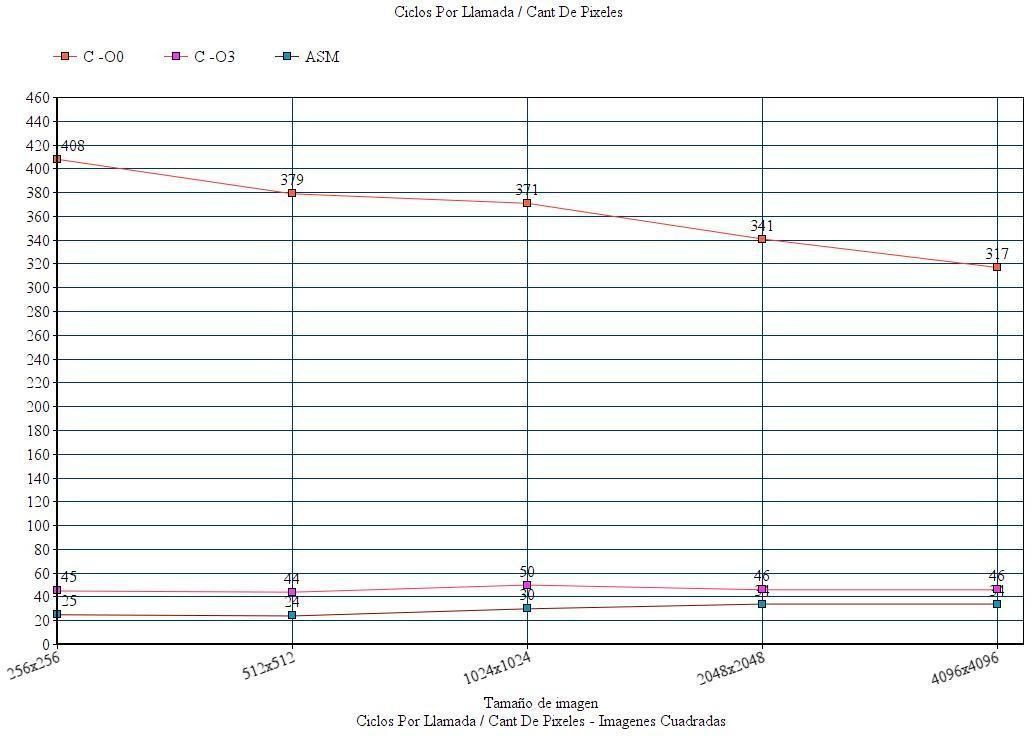
\includegraphics[width = 15 cm, height = 8 cm]{imagenes/ImgCuadradas.jpg}
	\caption[center]{Comparación diversas implementaciones - Imagenes cuadradas}
\end{figure}

\medskip
\begin{figure}[h!]
\centering
\captionsetup{justification=centering}
	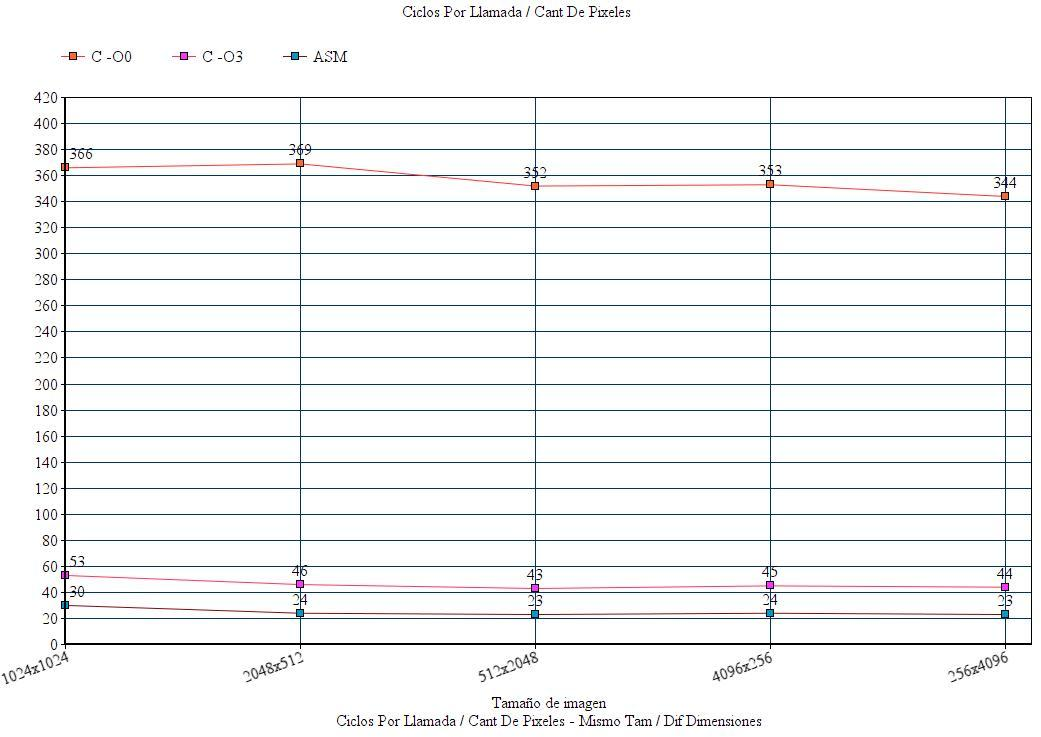
\includegraphics[width = 15 cm, height = 8 cm]{imagenes/DifDimensiones.jpg}
	\caption[center]{Comparación diversas implementaciones - Diferentes dimensiones }
\end{figure}

\medskip

\begin{figure}[h!]
\centering
\captionsetup{justification=centering}
	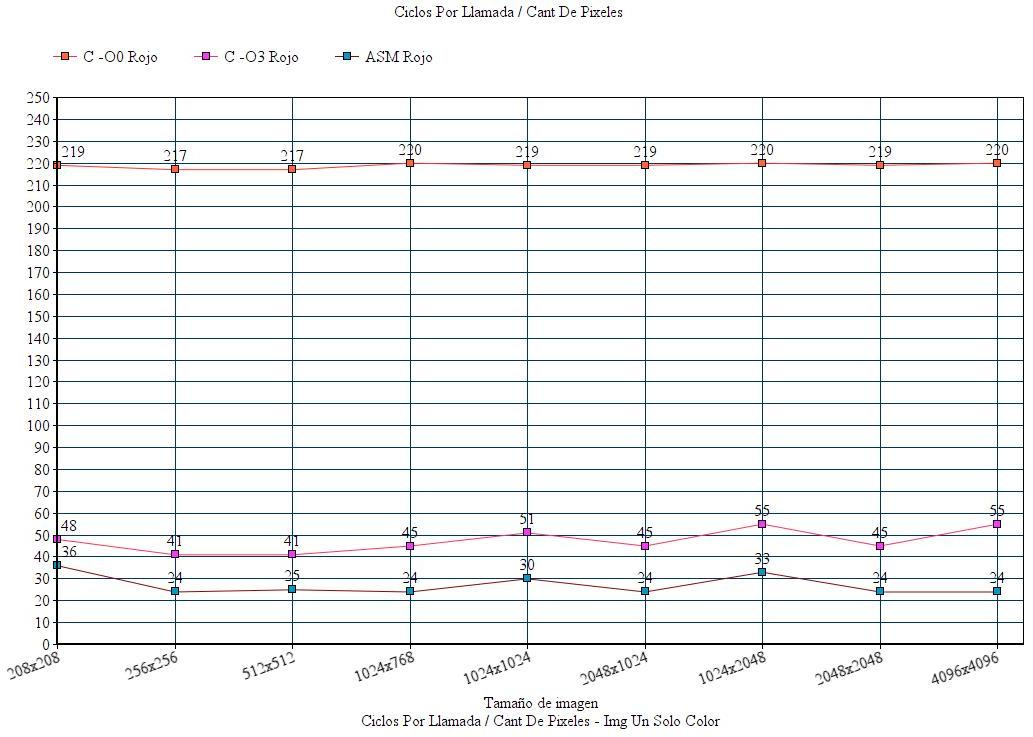
\includegraphics[width = 15 cm, height = 8 cm]{imagenes/mismoColor.jpg}
	\caption[center]{Comparación diversas implementaciones - Imágenes de un color}
\end{figure}

\subsubsection{Conclusión}
\par{La conclusión que podemos sacar de estos resultados es que, en primer lugar, como dijimos en la hipótesis, que se terminó corroborando, el código en C sin optimizar fue por lejos más lento que los otros dos. Y el código en C optimizado por más que mejoró muchísimo con respecto al anterior, siguió siendo más lento que el código en ASM.}
\par{Luego podemos ver que no nos confundimos tampoco en el momento de cambiar los tamaño de las imágenes pues los valores se mantuvieron casi constantes, justamente porque no se cambia la cantidad de operaciones que se hace respecto a las dimensiones de las imágenes, siempre se mantiene según la cantidad de píxeles.}
\par{Por último, nos llamó la atención el experimento de correr los códigos con imágenes de un solo color. Lo que pasó acá de extraño fue que las performance de los códigos en ASM y en C -O3 se mantuvieron iguales a los desarrollados con imágenes comunes, sin embargo el código en C -O0 demostró una gran mejora respecto a su performance, de la cual no podemos explicar precisamente el por qué, y de hecho esto también se ve en la primera imagen, donde para las imágenes de 4096x4096 el código en C -O0 mostró que mejoraba su rendimiento. Creemos que esto se debe a que justamente las imágenes que le pasamos tienen grandes secciones con píxeles del mismo color, porque son expansiones de una imagen de 512x512. Y se genera en estos fragmentos esta optimización que no podemos explicar sobre C -O0 en imágenes donde el color no cambia.}
	

\subsection{Experimentación 2}	

\subsubsection{Idea}
\par{El segundo experimento es un experimento más destructivo. Vamos a intentar molestar al jump predictor y ver cómo influye eso en la  performance del programa.}
\par{El experimento en sí trata de agarrar un número arbitrario desde los datos de entrada y en diferentes puntos de parada, ejecutar un control de flujo if then else, tal que dependiendo de \textcolor{red}{ciertas condiciones random de este número arbitrario}, salte a diferentes secciones del código. Todo esto dispuesto de tal manera que sea transparente a la ejecución final del programa, es decir, si el código sigue el camino del if no cambia a si sigue el camino del else.}

\subsubsection{Hipótesis}
\par{Nuestra hipótesis es que justamente el código no modificado va a ser bastante mejor que el código desarrollado con molestias para el jump predictor, porque en caso de funcionar estas, en cada ciclo estaríamos haciendo que flushee el pipeline, y que pierda muchos ciclos de clock extra.}
	
\subsubsection{Resultados}

\medskip\begin{figure}[h!]
\centering
\captionsetup{justification=centering}
	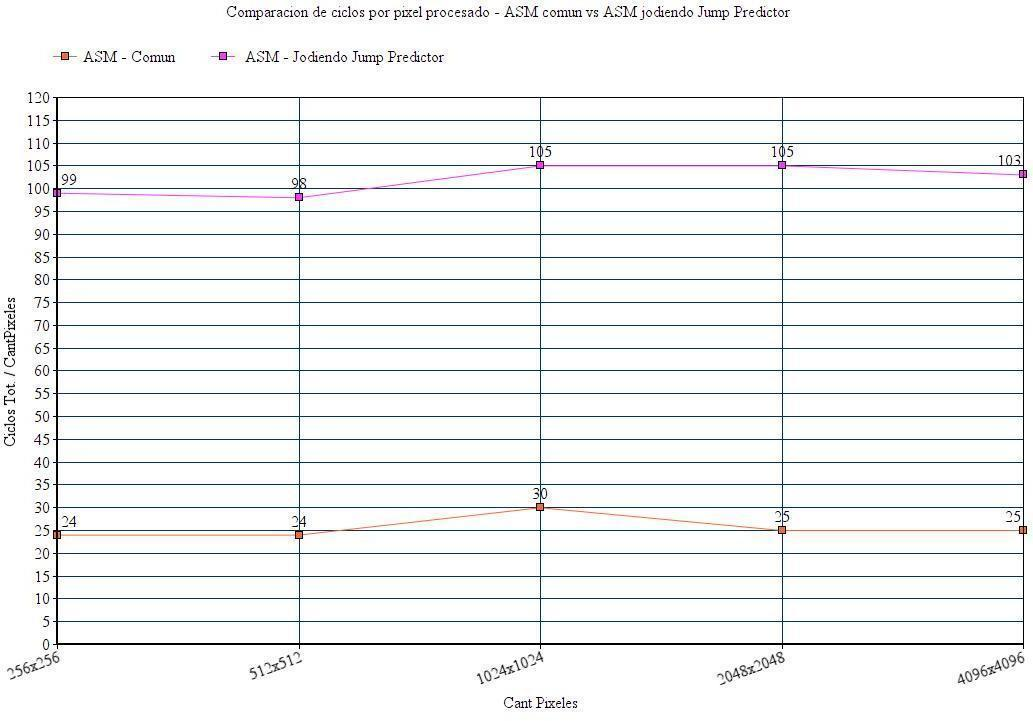
\includegraphics[width = 15 cm, height = 8 cm]{imagenes/JumpPredictor.jpg}
	\caption[center]{Comparación ASM comun vs ASM molestando Jump Predictor}
\end{figure}

\medskip

\subsubsection{Conclusión}
\par{Efectivamente los resultados fueron los esperados, por lo que nos llevamos como conclusión del experimento que influye mucho la arbitrariedad del flujo del \textcolor{red}{programa que se arma}. Si uno lo hace muy \textcolor{red}{aleatorio} como en este caso, por más que no afecte a la complejidad total el programa tarda significativamente más.}

\subsection{Experimentación 3}

\subsubsection{Idea}
\par{En el tercer experimento vamos a ver en qué medida es mejor aplicar la técnica de unrolling sobre un código. Lo que planeamos es correr el código de colorizar sobre una imagen de 1024x1024 desenrrollando el ciclo interior distinta cantidad de veces: vamos a empezar desenrrollando 16, luego 32, y luego completamente.}

	   
\subsubsection{Hipótesis}
\par{Lo que esperamos de este experimento es que el código desenrrollado 16 y 32 veces, mantenga el nivel de performance con el que demuestra normalmente, o resultados un poco más cercanos al óptimo, y esto se debe a que en sí el código de colorizar lleva muchas instrucciones, por lo que los pasos que nos ahorramos al desenrrollar el código no son significativos en el total del programa. Sin embargo en el caso de desenrrollar todo el código, esperamos una mucha peor performance por parte del código debido a que el tamaño del código aumentaría enormemente su tamaño de modo que no entrara en la memoria caché y debiera empezar a hacer lecturas de memoria para leer las instrucciones.}
	
\subsubsection{Resultados}

\begin{figure}[H]
\centering
\captionsetup{justification=centering}
	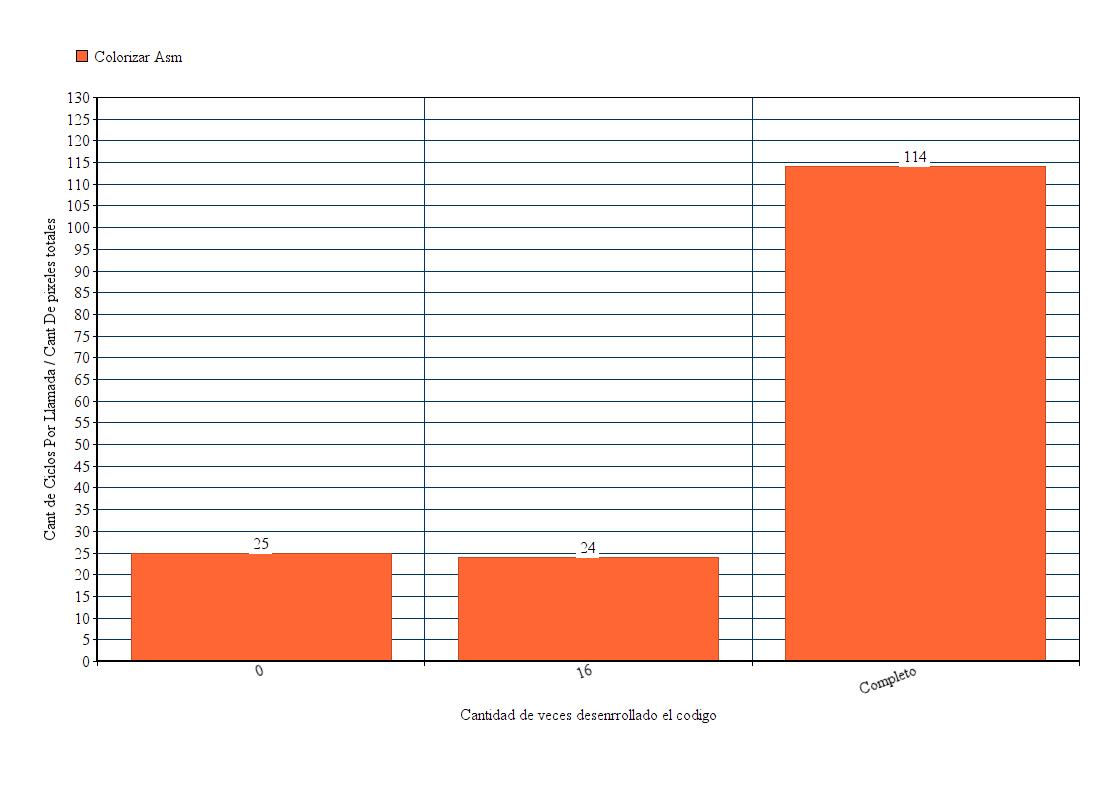
\includegraphics[width = 16.5 cm, height = 9 cm]{imagenes/unroll.jpg}
	\caption[center]{Comparación ASM común vs ASM unrrolling 16 vs ASM Unrrolling Completo}
\end{figure}
\medskip
	
\subsubsection{Conclusión}
\par{La conclusión que sacamos de este exprimento es que la técnica de desenrrollar código es efectiva para pequeños whiles, porque se eliminan algunas instrucciones inecesarias, sin embargo para un while de un tamaño mayor a lo usual, la optimización generada por esto se diluye hasta el punto de no notarse. Además de que efectivamente factores como la memoria caché son limitantes en esta situación, donde se da que los problemas de lectura de memoria dejan de ser parte de cómo es el algoritmo y pasa a ser a simplemente poder leerlo.}